%TEX root = ../dissertation.tex
\newtheorem{definition}{Definition}
\newtheorem{property}{Property}

\chapter{Background}
\label{chapter:background}

On this chapter, it is introduced some general concepts which are fundamental to
understand the problem at hand. These concepts are divided into three parts.
The first section concerns logical reasoning: starting from
\gls{FOL} and its role as inspiration for logical programming languages which
triggered the first wave of intensive \gls{AI} research and brought significant funding from both
public and private sectors, in the seventies. Then, it discussed a new framework
based on logical programming to describe uncertain domains called \gls{PLPL} and
its recent possible extension which uses dynamic distributional clauses. This
extension provides the ability to model
logical predicates as classical probabilistic distributions and also make them
vary along different time steps.\\
The second part focuses on decision and planning problems and finding optimal
ways to solve them if that is possible on polynomial complexity. It is also
discussed aproximate ways to solve them based on sampling. To finish this part,
the connection between \gls{PLPL} and planning is made along with all details
necessary to understand it.\\
Finally, on the third and last part of this chapter it is made a brief overview
of social robotics and its relation with symbiotic autonomy.

\subsection{Logical Programming}

Logical programming was the cause of popular excitement during the first wave of
\gls{AI}. It started in the late 60's and early 70's, when the first logical
programming languages were developed. \textit{Prolog} was one of those programming
languages. It currently sits as the 32nd most popular \footnote{According to the
 TIOBE index, October 2017} programming language.

\subsubsection{Prolog}
\textit{Prolog} is a logical programming language first introduced by Alain Colmerauer
and Philippe Roussel \cite{Colmerauer1993}, in 1972, that was designed to simulate
the man-machine communication system in natural language. The goal was also to
integrate logic as a declarative knowledge representation language with a
procedural representation of knowledge.

The ensemble of facts \ref{pl:fact}, clauses \ref{pl:clause} and queries are built out of terms, its single data
type. Terms can be complex or simple, if they are composed by logical variables or
constants (Atoms or Numbers). Variables start with an upper case letter while constants 
start with a lower case letter.
As it is said before, what makes this programmming language different than
others is the fact that it is declarative, it does not describe the control flow
of the program, only the logic of the computation. This logic is expressed by
means of relations between objects, and its execution is started by running a
query over the program's knowledge base. Programs are compiled by using a
combination of facts and clauses which are in turn,
transformed to a knowledge base \ref{pl:kb}.

\begin{definition}[Clause]
    Is a first order formula, represented by an
    implication clause that is read from the right to the left. The leftmost
    member is called the \textit{Head}
    and the set of facts to the right are called the \textit{Body}. This
    \textit{Body} can contain both disjunctions and/or conjuctions of facts.
    \label{pl:clause}
\end{definition}

\begin{definition}[Fact]
Is a grounded (no variables) clause with an empty \textit{Body}.
  \label{pl:fact}
\end{definition}

Examples of a fact and a clause are shown in \ref{pl:prolog_clause} and \ref{pl:factex}, 
respectively.

\begin{equation}
    location(O, X) \leftarrow has(Y, O), location(Y, X).
    \label{pl:prolog_clause}
\end{equation}

\begin{equation}
    robot(mbot).
    \label{pl:factex}
\end{equation}

\begin{definition}[Knowledge Base]
    It is a collection of facts and relations which are loaded into program's
    memory, when it is executed.
    \label{pl:kb}
\end{definition}


New rules can be created by joining a combination of facts, increasing the
information about the world.
It is also important to know that when a prolog program is started, it loads all
the clauses and facts into its Knowledge Base. Then, to interact with it, the
user needs to query it. These queries can be completely grounded, with variables
or even containing both the terms.
The query provided to the prolog interpreter is
handled through the rules and facts present in the knowledge base using the
Unification-Resolution mechanism with a backtracking flow model control,
returning 'Yes', if the solver can prove the query clause with all the remaining
clauses in the database, or 'No', if the solver cannot prove it with the
available information about the world.
It can also show all the possible unifications with variables it found while
running that same query.

It is also important to mention that Prolog is built upon the
\textit{Closed World Assumption}, which says that all knowledge about the world
is present in the database. The result provided by the
interpreter must be seen as an attempt of the programming language to prove that
the asked query is true in some model of the world. So if the solver returns a
'No' answer, it does not necessarily mean that the query clause is false, just
that the solver cannot prove it with the available information about the world.

A simple prolog example relevant to the problem that is being treated can be
seen in snippet \ref{pl:example1}.

\begin{gather}
  robot(mbot).\nonumber\\
  object(coke).\nonumber\\
  region(kitchen). \nonumber\\
  region(bathroom). \nonumber\\
  has(robot, coke). \nonumber\\
  located(mbot, kitchen).
  \label{pl:example1}
\end{gather}

From the previous simple program, it is interesting to make multiple queries
about its knowledge base. One can query \textbf{?- region(X)}, in order to get
every possible region term. It is also possible to query about the robot
location, \textbf{?- located(mbot, X)}; in this case, the answer is obvious,
as there is already an explicit fact about it in the knowledge base. But,
imagine the location of the coke is also important for the problem. Since the
robot has the object, its location will be the same. So, in order to replicate
the previous behaviour, the following clause was introduced into the knowledge
base.

\begin{gather}
  located(X, Y) \leftarrow has(A, X), robot(A), located(A,Y).\nonumber\\
  \label{pl:example2}
\end{gather}

It is now possible to get information about coke's location.

There are currently multiple \textit{Prolog} implementations and each one has its
own advantages, limitations and support. Currently, the most popular are
\textit{SWI Prolog} and \textit{Yap Prolog}\footnote{The latter can be found in
\url{http://www.swi-prolog.org/} and the former in
\url{https://www.dcc.fc.up.pt/~vsc/Yap/}}. The work developed along this
thesis uses the latter.

A good book on \textit{Prolog} and logic programming in general is
\cite{nilsson1990logic}, which should be consulted in order to get more
information about this topic.

\subsection{Probabilistic Logical Programming}

\subsubsection{\glspl{DC}}

\glspl{DC} \footnote{Implementation by Davide Nitti is available on
\url{https://github.com/davidenitti/DC}} \cite{nitti2014relational}
\cite{nitti2016probabilistic} - inspired by Sato's Distribution Semantics \cite{sato1995statistical} - 
are an extension of logic programming which can
represent random variables as probability distributions. It includes typical
probability distributions: \textit{uniform}, \textit{gaussian},
\textit{discrete finite choice}, \textit{poisson}, \textit{beta}, etc.
The formal syntax of \glspl{DC} are normal \textit{Prolog} definite clauses, but
with few addons:

\begin{equation}
    x \sim D \leftarrow b_1, ..., b_n.
    \label{pl:dc_clause}
\end{equation}

Where $x$ is the random variable, represented as a \textit{Prolog} term; $D$ is
the probability distribution, which can also include other terms. Until now,
every term explained is contained on the head of the clause. But \glspl{DC} also
include a body: $b_1, ..., b_n$, where $b_k$ are literal terms.
The body should have a valid substitution in
order to generate variable $x$, and each grounding of the body will generate an
instance of $x$. These special clauses can also include logical variables
(when written in capitalized format) in
both the body and the head, giving it an higher dimension of abstraction.

Another important detail is the operator $\simeq$, in snippet \ref{pl:dc_simeq},
which is used to get the outcome of some randomly distributed variable.

\begin{equation}
    y \sim val(true) \leftarrow \simeq(x) = true.
    \label{pl:dc_simeq}
\end{equation}

After adding some \glspl{DC} into a \textit{Prolog} program, it is now called
a distributional program. The program will generate a distribution over possible
worlds from the information given by all clauses in the \gls{KB}. The inference
procedure is the following:
\begin{enumerate}
  \item Initialize possible worlds, $W$, as an empty set;
  \item For every \gls{DC}, find an unique substition of the body and if it is
  possible, sample a value from the head's distribution and add it to $W$.
  \item If it is impossible to generate more worlds, the program ends.
  \item It is now possible to make probabilistic inferences from the sampled
  world.
\end{enumerate}

After all the above steps are complete, probabilistic inferences are made by
querying the \textit{Prolog} program over all possible worlds.

An example of a distributed clause describing the robot location is shown in
\ref{pl:dc_example}. It models the robot location as a random variable and it is
governed by a uniform distribution of possible values. On this case,
the values are regions: kitchen, bed and sofa.

\begin{equation}
    location(robot) \sim uniform(kitchen, bed, sofa) \leftarrow true.
    \label{pl:dc_example}
\end{equation}

\subsubsection{Dynamic Distributional Clauses}

\glspl{DDC} \cite{nitti2016probabilistic} adds more expressiveness to \glspl{DC}
by introducing temporal
modeling. This is done by adding a subscript \ref{pl:dc_temp_clause} to the
previously defined random variables. This way, it is possible to describe
logical interpretations that can evolve over time periods. In order to have this
kind of dynamic clauses, random variables just need to have a time index
associated with their program terms.

\begin{equation}
    x_{t+1} \sim D \leftarrow b_1, ..., b_n.
    \label{pl:dc_temp_clause}
\end{equation}

In order to have a correct \textit{Prolog} program with \glspl{DDC}, the random
variables must be defined:
\begin{itemize}
  \item in the initial timestep, $t=0$,  also known as the prior distribution.
  \item the transition model, which describes how a random variable evolves
  through successive time steps.
\end{itemize}

Example \ref{pl:dc_example} can now be extended with the proper model, as seen
in \ref{pl:dc_example2}. So, the robot will always be in the same place as time
passes.

\begin{equation}
    location(robot)_{t+1} \sim val(X) \leftarrow \simeq(location(robot)_t) = X.
    \label{pl:dc_example2}
\end{equation}


\subsubsection{Related Methods}

The prime example of a \gls{PLPL} is \textit{Problog} \cite{de2007problog} from \textit{De Raedt et al.}
The authors devised the programming language as a probabilistic extension of the original 
\textit{Prolog}. On this language, a \textit{Problog} program defines a distribution over 
\textit{Prolog} programs. Also, each clause specifies the probability of belonging to a randomly 
sampled program. The ultimate goal is to make probabilistic inferences by running \textit{Problog}
queries into the \gls{KB}. 
In contrast with \glspl{DDC} which are used in these work, \textit{Problog} lacks sampling from
probability distributions and builtin support for timed logical interpretations.

Another interesting work was done by \textit{Milch et al.} in \cite{milch20071}. 
They proposed and developed a language syntax in order to procedurally describe probabilistic models
that have an unknown number of objects. The language is called BLOG (from \textit{Bayesian Logic}) and
it is able to handle bayesian models in a compact manner. An inference engine was also developed based
on sampling methods over possible worlds.

\section{Decision Theory and Planning}

\subsection{Markov Decision Processes}

It is important to formalize a model that can capture the uncertainty contained
on domestic environments with robots. These robotic agents must make optimal
decisions (or approximately optimal) while knowing that their actions can
possibly lead to multiple exclusive outcomes.

A classical method is to formalize these domains as \glspl{MDP}
\cite{Sutton1998} \cite{bertsekasneuro} \cite{russell1995modern}.
This kind of processes have been extensively studied by Decision Theory
research and have a broad range of applications: economics, routing, general
game playing, operations research and also robotics, of course.

An interesting feature of \glspl{MDP} is that information about the current
state is sufficient to completely characterize the decision problem at the current
step. However, it is important to remark that while these models can capture the
uncertainty of the world, it must come from probabilistic outcomes of actions
and not from the current state. Models that can incorporate
uncertainty on the current state are called \glspl{POMDP}, although they will
not be featured on this work.

A process of this genre has a set of states, $S$, which can be discrete: finite
or infinite; or continuous. Along the current work, the spotlight is on discrete
states, although the proposed framework is expressive enough to handle
continuous states.

In order to transition from one state to another, the agent
uses an applicable action from the action space, $A$. When the agent transitions
to a new state, it receives a reward, returned as a function of its current
state, action taken at this step and also the new transitioned state.

The main law of this processes is the so called Markov Property
\ref{def:markov_property} which mathematically translates what has been said
earlier.

\begin{property}[Markov Property] The conditional probability of future state
depends exclusively on the current state and it is independent of all previous
states.
\label{def:markov_property}
\begin{equation}
    P(s_{t+1}|s_{t}) = P(s_{t+1}|s_{t},...,s_1)
\end{equation}
\end{property}

In order to fully capture information given by the model and
explicitly introduce the fact that the agent has to make decisions, it is
necessary to make a generalization for \glspl{MDP} \ref{def:markov_process} of
\ref{def:markov_property}.

\begin{definition}[Markov Process]
    A process where \ref{def:markov_property} holds is called a Markov Process.
    On these processes, the following equation holds:
    \begin{equation}
        P(s_{t+1}|s_{t}, a_{t}) = P(s_{t+1}|s_{t},a_{t}...,s_1, a_1)
        \label{eq:markov_property_action}
    \end{equation}
    \label{def:markov_process}
\end{definition}

The probabilities given by \ref{eq:markov_property_action} are known by state
transition probabilities and are commonly represented on a matrix, if the
state-action space is countable and finite. Under the assumption of
\ref{eq:markov_property_action}, all the past history of states and actions is
irrelevant in order to find the next state the agent will be in, when it
executes some specific action. It only depends on the current state.

\begin{definition}[Markov Decision Process]
    A process where an agent has to make decisions and \ref{def:markov_process}
    holds. It is characterized by $<S, A, T, R>$:
    \begin{itemize}
        \item $S$, set of states.
        \item $A$, set of possible actions.
        \item $T$, state transition model.
        \item $R$, reward function.
    \end{itemize}
\end{definition}

A simplified version of this thesis \gls{MDP} is shown in figure
\ref{fig:mdp_example}. This short example shows how \glspl{MDP} can describe
domestic environments with robots.

\begin{figure}[H]
    \centering
        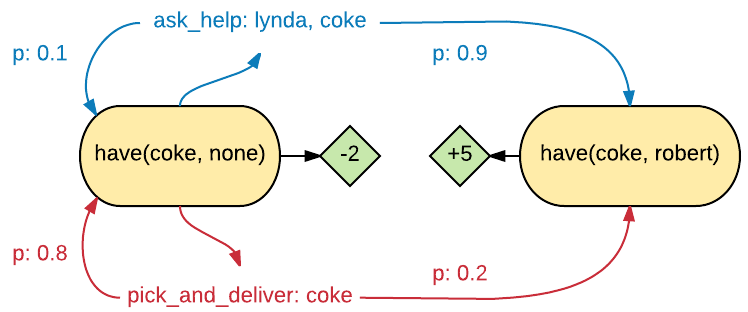
\includegraphics[width=11cm]{images/mdp_example}
        \caption{Overview of a simple Markov Decision Process for domestic environments,
        described for the robotic agent. There are only two states in this
        process, and they are colored yellow. Actions are colored blue and red and
        have the same cost. Outcomes of each action are enumerated from its name
        along with its explicit probability of occurring. Rewards are obtained
        when the robot reaches each individual state and are represented as
        green diamonds with respective values inside.}
        \label{fig:mdp_example}
\end{figure}

\subsection{Solving Markov Decision Processes}

Having the problem statement formally defined, it is now time to discuss on how
to solve them. The objective here is to maximize the
\textit{Return} \ref{def:return} from the current state to the goal or on a
specified horizon.

\begin{definition}[Return] defined as the discounted reward from the current
    state, while following some policy \ref{def:policy}, on a specified number
    of steps, infinite or finite. $\gamma$ is the discount factor and it is
    bounded between 0 and 1.
    \begin{equation}
        G_t = \sum_{k=0}^{\infty} \gamma^{k} r_{k}
        \label{eq: mdp_return}
    \end{equation}
    \label{def:return}
\end{definition}

The discount factor $\gamma$ can make the rewards awarded far into the future
less valuable. This factor is meant to simulate inflation as it appears in economics.
It motivates the agent to take actions that lead to increased immediate rewards.
In parallel, it is also a way of overcoming the difficulty of planning on a
infinite horizon.

\begin{definition}[Policy] is a function $\pi(a|s)$, which gives the probability
      that an agent has of taking action $a$ while on state $s$. A policy can
      also be deterministic, if in every state there is one and only one action
      with probability equal to one.

      \textit{An example of an optimal policy which is stochastic: Paper, Rock
      and Scissors game, or guessing the result of a coin flip.}

      A policy can be classified as:
      \begin{itemize}
        \item \textbf{Complete: } if there is a mapping for every state in $S$.
        \item \textbf{Partial: } if a policy is not complete.
        \item \textbf{Closed: } if an agent starting from the current state, $s_0$,
        is able follow the current policy without ever needing to replan.

      \end{itemize}

      \label{def:policy}
\end{definition}

It is now appropriate to talk about the concepts of State-value \ref{def:value}
and Action-value \ref{def:q_value} functions and how closely are they tied with
the current policy. Using loose terminology, they are a measure of how
\textit{good} a state is for the agent, while following some particular policy.

\begin{definition}[State-value function] is the expected long term return of a
    state $s$ while following some policy $\pi$ on the following future.
    \begin{equation}
        v_{\pi}(s) = E_{\pi}\Big[ G_t | S_t = s \Big]
    \end{equation}
    \label{def:value}
\end{definition}

\begin{definition}[Action-value function] is the expected long term return of a
    state $s$ and after taking some action $a$, while following some policy
    $\pi$ on the following future.
    \begin{equation}
        q_{\pi}(s, a) = E_{\pi}\Big[ G_t | S_t = s, A_t = a \Big]
    \end{equation}
    \label{def:q_value}
\end{definition}

\subsection{Dynamic Programming}

The goal of solving \glspl{MDP} is to find the Optimal Policy
\ref{def:opt_policy} for every possible state. One way to find it, is by using
dynamic programming. Basically, it is a method for solving complex problems by
turning them into subproblems and combining the solutions of them. Since these
subproblems occur many times, one can cache their result and reuse it to solve
the main problem.

\begin{definition}[Optimal Policy], $\pi^*$ is a Policy which has the highest
state-value function possible for a particular problem, the optimal State-value
function.
It is also important to mention that it can exist multiple optimal deterministic
policies for the same optimal State-value function.
\label{def:opt_policy}
\end{definition}

So, equation \ref{eq:bellman_backup} is used to dynamically solve \gls{MDP}. It is
normaly called the \textbf{Bellman Equation} for $v_{\pi}$. Another equivalent
equation exists for $q_{\pi}$. Using the latter provides faster convergence, but
an higher amount of memory used. This happens because one has to store more values
for the combination of state and possible applicable actions than just storing
values for each state, exclusively.

\begin{equation}
    v_{\pi}(s) = \sum_{a \in A} \pi(a|s) \sum_{s' \in S} p(s'|s,a)
    \big[r(s',a,s) + \gamma v_{\pi}(s') \big]
    \label{eq:bellman_backup}
\end{equation}

In order to better understand how \ref{eq:bellman_backup} makes the update of
the state-value and action-value function, it is usual to draw a tree diagram,
the \textit{Backup Diagram} \ref{fig:backup_diagram}, which encompasses these
variables across successor states from the root, the initial state $s_0$. It is
organized in successive layers of $v_{\pi}^k$ until a goal or the end of an
horizon is reached.

\begin{figure}[H]
    \centering
        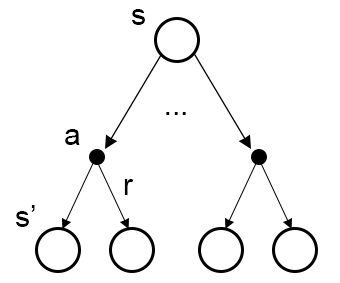
\includegraphics[width=4cm]{images/backupdiagram}
        \caption{Backup diagram of dynamic programming while using Bellman
        Backups.}
        \label{fig:backup_diagram}
\end{figure}

It happens that finding an optimal policy for a \gls{MDP} is a task which can be
done in polynomial time \cite{littman1995complexity} when formulated as a linear
program. Though, due to the curse of dimensionality, the order of these
polynomials can be so high that it is impractical to get efficient solutions.
Also getting an optimal policy for all the state space on a \gls{MDP} is a
P-complete problem \cite{second_complexity}.

The classical method to solve \glspl{MDP} is based on this programming paradigm.
It is recognized by the name of Value Iteration \ref{subsection:value_iteration}.

\subsubsection{Value Iteration}
\label{subsection:value_iteration}

This algorithm \cite{bertsekas1987dynamic} is based on the Bellman Optimality
Equation \ref{eq:bellman_optimal}.

\begin{equation}
    v^*(s) = max_{a \in A} \sum_{s' \in S} p(s'|s,a)
    \big[r(s',a,s) + \gamma v^*(s') \big]
    \label{eq:bellman_optimal}
\end{equation}

The line of reasoning is to iteratively run
the previous equation for every state in the \gls{MDP}. This complete procedure
is repeated until some condition is verified. The usual conditions are:
\begin{itemize}
  \item \textbf{$\theta$-convergence algorithm} \ref{alg:theta_conv}. It just
  compares the current state-value function for the current iteration with the one
  at the previous step. If some state has state-value bigger than $\theta$, then
  it has not $\theta$-converged yet;

  \begin{algorithm}[H]
      %\BlankLine
      \DontPrintSemicolon
      \SetKwInOut{Input}{input}
      \Input{State space $S$. \newline State-value functions $V_{k}$ and $V_{k-1}$
      .}
      \ForAll{s in $S$}{
          \If{$ V_k[s] - V_{k-1}[s] > \theta $}{
              \Return{False}\;
          }
      }
      \Return{True}
  \caption{$\theta$-convergence of the state-value function of \gls{MDP}.}
  \label{alg:theta_conv}
  \end{algorithm}

  \item \textbf{Maximum number of iterations};
  \item \textbf{Timeout}.
\end{itemize}

\begin{algorithm}[H]
    %\BlankLine
    \DontPrintSemicolon
    \SetKwInOut{Input}{input}
    \SetKwInOut{Output}{output}
    \Input{\gls{MDP}, $<S, A, T, R>$. \newline
            $\theta$, convergence threshold.\newline
            $\gamma$, discount factor.
            }
    \Output{$\pi^*$, the $\theta$-optimal policy. \newline
            $V^*$, the $\theta$-optimal state-value function.
    }
    $ k \gets 0 $

    $ \forall s \in S, V_{k}^*(s) \gets 0$

    \Repeat{ $V_{k}^{*}$ has $\theta$-converged}{

        $ k \gets k + 1 $

        \ForAll{s in $S$}{
            $ V_{k}^{*}(s) = \max_{a \in A}\sum_{s' \in S} p(s'|s,a)[r(s',a,s) +
            \gamma V_{k-1}^{*}(s')]$
        }
    }

    \ForAll{s in $S$}{
        $\pi^*(s) = argmax_a \sum_{s' \in S} p(s'|s,a)[r(s',a,s) +
            \gamma V_{k-1}^{*}(s')] $
    }

    \Return{$\pi^*$, $V_{k}^{*}$}
\caption{Value Iteration for a generic \gls{MDP} with the $\theta$-convergence
criteria.}
\label{alg:value_iteration}
\end{algorithm}

\par

The Optimal Policy can only be obtained with full certainty, if one is using the
$\theta$-convergence criteria and $\theta$ parameter is set to zero. However,
this is not always possible, as the number of states can be too large or there
are time constraints to solve the \gls{MDP}. One way to deal with these
constraints is by using \gls{RL} techniques as seen in the following section.

\subsection{Monte Carlo Learning}

Unlike algorithm \ref{alg:value_iteration} which is based on dynamic programming,
\gls{MCL} \cite{Sutton1998} is a sample based method that involves learning the
optimal policy from episodic experience. Additionally, it does not even need an
explicit model of the world (i.e., the transition model and the reward
function). Though, a blackbox simulator of it is needed. Figure
\ref{fig:mcl_agent} describes an agent following this behaviour. The agent's job
is to find and execute the best action, given the current situation. Afterwards,
the simulator gives a sample of the new state and a reward. This process
is repeated until it fulfills some previously defined condition.

\begin{figure}[H]
    \centering
        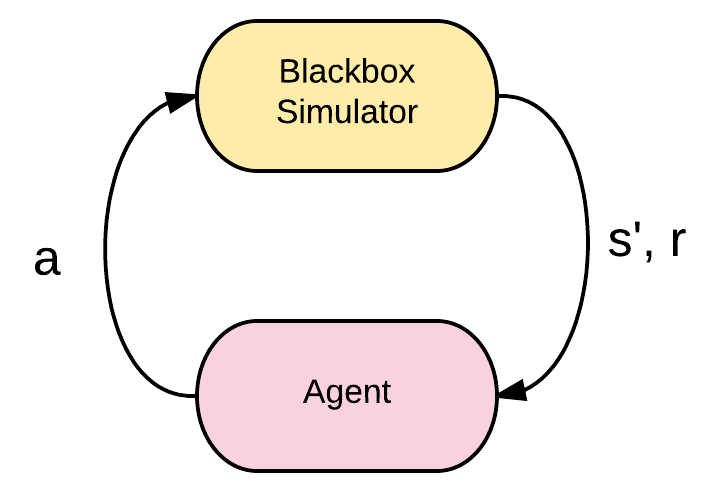
\includegraphics[width=6cm]{images/MCL-model}
        \caption{Schematic of a \gls{RL} agent operation.}
        \label{fig:mcl_agent}
\end{figure}

Again, it is not possible to deterministically calculate the state-values, as
the model is unknown to the agent, so he must resort to estimates, using the sum
of the rewards gained on every episode containing this state, averaged over
all the completed episodes which have that same state.

Moreover, since the agent is trying to find the optimal policy, he should not always
take actions which give him the best expected rewards, as the state-values can
have a high amount of bias in them. So, he must mix exploitation of the current
policy with exploration of unknown states in order to converge to the optimal
policy.

This computational paradigm has been
followed in many successful \gls{RL} algorithms, like \textit{Q-Learning} and
\textit{SARSA} \cite{Sutton1998} and more recent ones using Deep Neural Networks
like \textit{Deep Q-learning} \cite{mnih2015human} \cite{mnih2013playing}.

\subsection{Factored Markov Decision Processes}
When learning the theory behind \glspl{MDP}, it is often easier to describe
them using its explicit representation. It is called explicit because the
transition probabilities are discriminated for every possible state
of the world model. The same applies for goals and actions.

However, this type of representation does not scale to bigger problems, as the
state space is often too big to be enumerated.
So, an alternative way to model \glspl{MDP} exists, and the reasoning behind it
is to represent each state by a combination of multiple attributes of the world
model.

This representation was introduced by \cite{boutilier1999decision}. On this
specification, each state is composed of multiple factors, normally referred as
state variables. Each factor has its own domain and the total space size is the
combination of all possible values for each state variable.

The main advantage of having this kind of representation is that each
probabilistic transition can be separately represented by a \gls{DBN}.

In order to understand what a \gls{DBN} is, one must explain what is a \gls{BN}.
\glspl{BN} are a class of probabilistic graphical models which represent
dependencies of variables with directed graphs. It contains nodes, which
represent state variables, and edges between them, expressing a causal
dependency between them.
Every node has a conditional probability table that expresses these relations
mentioned above. A \gls{BN} can represent a set of factored models that are
time invariant. If a temporal dependence exists, \glspl{DBN} can be used to
model them. They are represented as a two step \gls{BN}, one on the current time
step and the other on the next time step, with the same variables on each.
Temporal dependences are represented by edges from variables on the first
timeslice to variables on the second timeslice. There is not any edge between
variables on the first time step. However, it can exist edges between variables
on the second time step. They are meant to represent effects that have a
common cause.

These factored representations are used to describe the domains further along
this thesis. An example of a factored MDP, which was actually used to model the
location of the robot in the house is showed in \ref{fig:fmdp_example}:

\begin{figure}[H]
    \centering
        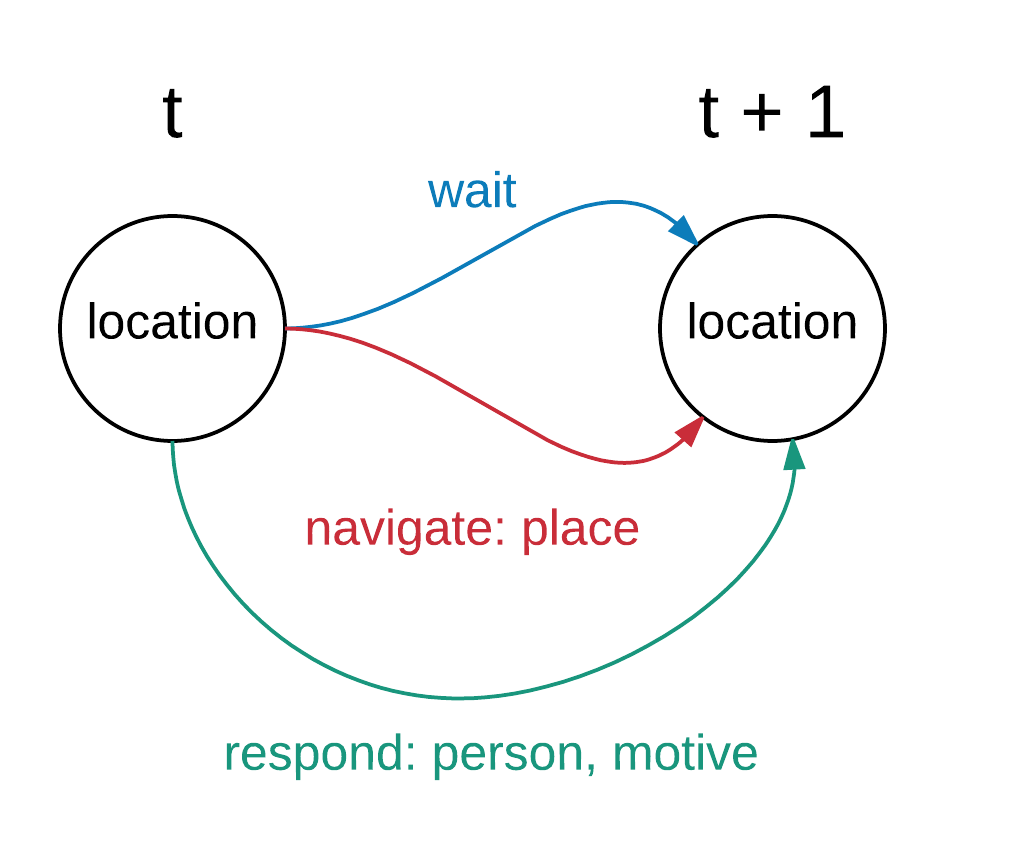
\includegraphics[width=6cm]{images/fmdp}
        \caption{\gls{DBN} describing part of the factored Markov Decision Process for the
        robot. The illustrated state here is the robot location. It can be
        either of these three values: "kitchen table", "sofa" or "bed".}
        \label{fig:fmdp_example}
\end{figure}

\subsection{\gls{HYPE} Planner}

While searching for an appropriate planner that would take advantage of logical
programming, multiple options were possible \ref{subsubsection:rlpp}.
But, in the end, the choice fell upon \gls{HYPE} algorithm
\cite{nitti2015planning} (pseudocode is shown in \ref{alg:hype}), a state of the
art planner completely written in
\textit{Prolog}. Some of its most important features include domains
with an unknown number of variables and handling both discrete and continuous state
and/or action spaces. All of this is accomplished after describing the domain,
using \glspl{DDC} on a \textit{Prolog} program, and following a set of syntax
rules (see section \ref{subsubsection:correct_domains} for more information about
these rules).

Unlike other classical algorithms based on dynamic programming
\ref{alg:value_iteration}, \gls{HYPE} takes advantage of \gls{MCL} in order to
overcome the curse of dimensionality and build the state-value function.
Since others that follow this approach do not use information about the
transition model, \gls{HYPE} incorporates importance sampling in order to take
advantage of that same model.

Also, and similarly to \textit{Q-learning} \cite{Sutton1998}, it follows an
off-policy strategy to update the state value function. This means that the
value of the optimal action is learnt without following the current policy.
Its implementation uses an $\epsilon$-greedy strategy to sample an action
from the current state, i.e. with probability $p$ chooses the action with the
highest action-value estimate, otherwise, samples a random action according to an
uniform distribution.

The algorithm takes advantage of logical interpretations for representing
states in the domain. These logical interpretations are ground facts that
define a possible world.

\begin{algorithm}[H]
    %\BlankLine
    \DontPrintSemicolon
    \SetKwInOut{Input}{input}
    \SetKwInOut{Output}{output}
    \SetKwProg{Fn}{Function}{}{}
    \Fn{HYPE\_recursive ($d$, $s_t^m$, $m$)}{
    \Input{$d$, horizon. \newline
            $s_t^m$, state of the world at timestep $t$ in episode $m$.\newline
            $m$, episode number.
            }
    \Output{$V^m(s_t)$, the state-value estimate for $s$ in episode $m$.}

    \If{ d = 0}
    {
      \Return{0}
    }

    \ForAll{action $a$ in applicable($s_t^m$)}{
        $ Q_d^m(s_t^m,a) = r(s_t^m,a) + \gamma \frac{\sum_{m \in M} w^m V_{d-1}^m(s_{t+1}^m)}{\sum_{m \in M} w^m}$
    }

    $ a_t^m \gets \epsilon$-greedy($s_t,Q_d^m$)

    Sample $ s_{t+1}^m \sim T(s_{t+1}| s_t^m, a_t^m) $

    $ V_d^m(s_t^m) \gets r(s_t^m, a_t^m) + \gamma$ HYPE\_recursive($d-1$, $s_{t+1}^m$, $m$)

    Put in memory $ (s_t^m, V_d^m(s_t^m),d) $

    \Return{$V_d^m(s_t^m)$}

    }
\caption{\gls{HYPE} algorithm for solving \gls{MDP} problems, as shown in
\cite{nitti2015planning}.}
\label{alg:hype}
\end{algorithm}

\subsubsection{Implementing \gls{HYPE} Domains \& Problems}
\label{subsubsection:correct_domains}

In order to write a syntactically correct \gls{HYPE} domain, it is necessary to
follow some rules:
\begin{enumerate}
  \item Decide whether is preferable to use an implicit or explicit
  representation of the \gls{MDP}. If an explicit model is chosen, there only
  exists one predicate at each timed step.
  \item Identify needed predicates which are necessary to describe the \gls{MDP}
  and goal predicate(s). Imagine, for example, that an agent has the goal of
  reaching the kitchen:
  \begin{equation}
    stop_t \leftarrow \simeq(location(agent)_t) = kitchen.
  \end{equation}
  \item Enumerate all possible actions in the domain and explain when they are
  available to be used. Actions should describe what states they are
  applicable. A simple example is shown below, describing when the action
  deliver is available to be used:
  \begin{equation}
    applicable(deliver(coke, lynda))_t \leftarrow \simeq(have(coke)_t) = agent,
        \simeq(near(lynda)_t) = true.
  \end{equation}
  \item Choose the proper rewards: they can be function of specific interpretation
  \ref{eq:log_rew1}, action \ref{eq:log_rew2} or even both \ref{eq:log_rew3}. It
  can also be used to give a reward when the goal is reached \ref{eq:log_rew4}.
  Though, it is important to mention that rewards are mutually exclusive. So,
  this can be a serious limitation if the domain designer chooses a factored
  state representation.
  \begin{equation}
    reward(10)_t \leftarrow \simeq(have(coke)_t) = lynda.
    \label{eq:log_rew1}
  \end{equation}
  \begin{equation}
    reward(-10)_t \leftarrow deliver(coke, lynda)_t.
    \label{eq:log_rew2}
  \end{equation}
  \begin{equation}
    reward(-4)_t \leftarrow \simeq(near(lynda)_t) = true, deliver(coke, lynda)_t.
    \label{eq:log_rew3}
  \end{equation}
  \begin{equation}
    reward(10)_t \leftarrow stop_t.
    \label{eq:log_rew4}
  \end{equation}
  \item Describe the transition model of the domain using \glspl{DDC}. It uses a
  structure similar to \textit{Situation Calculus}. So, when
  some action is executed, it must dictate what will change and also what
  remains the same. An example is, for instance, the movement action of an agent
  and its effects on others around him:
  \begin{equation}
    location(agent)_{t+1} \sim finite([0.8:hall, 0.2:kitchen]) \leftarrow action(navigate(hall)).
    \label{eq:log_trans1}
  \end{equation}
  \begin{equation}
    location(lynda)_{t+1} \sim val(Region) \leftarrow action(navigate(Y)), \simeq(location(lynda)_t) = Region.
    \label{eq:log_trans2}
  \end{equation}

  \item Instatiate a problem by grounding the current predicates with their
  respective values or probability distributions.
  \item Try to find which hyperparameters (episode horizon, discount factor,
  exploration bias, number of episodes, etc) give the best domain results
  by differential parameter tuning under simulation benchmarks.
\end{enumerate}


\subsection{Related Logical Probabilistic Planners}
\label{subsubsection:rlpp}

In \cite{van2010dtproblog}, \textit{den Broeck et al.} presented a decision theorethic extension of
\textit{Problog} with the name \textit{DT-Problog}. It included a set of syntax rules that was 
expressive enough to describe simple planning problems. It includes two integrated algorithms for
solving them: an approximate solver which is faster but non-optimal; and an exact one which can 
take a lot longer in order to converge. They express actions as \textit{decision facts} and rewards
as utility attributes. However, the language lacks expressiveness in order to efficiently solve 
sequence of temporal decision episodes. Also, it does not support continuous facts and decisions which
can be essential in robotics problems.

Another related approach is proposed in \cite{lang2010planning} by \textit{Land and Toussaint}.
They make use of \textit{Noisy Indeterministic Deictic} rules in order to learn abstract representations
of the world. In turn, those rules are integrated into a planner by the name of \gls{PRADA}, which was
developed by the same authors and takes advantage of probabilistic inference in order to handle 
probabilistic action effects. Finally, this architecture was applied into a 3D manipulation task and
likewise to the domains of \gls{ICAPS-IPC}.

\section{Social Robotics}

\subsection{Domestic Robots}
\label{sec:dom_robots}

There have been a lot of attempts to introduce robots in domestic environments.
But the most successful case is in vacuum cleaning industry. There are now
multiple inexpensive robots that autonomously clean house floors. Still, the
majority of interesting tasks in household domains are incredibly difficult to
perform in real scenarios within tight schedules.

Tasks in domestic environments integrate multiple skills like perception,
grasping or others which are incredibly difficult to perform on separate benchmarks.
Normally, they have high accuracy but are not time efficient or even the other way around.
Robot grasping is one of those skills, but with other problems: reliable robotic
manipulators are not affordable to the average citizen. The problem here is that
most of these tasks requires the robot to interact physically with one or more
objects in the scene.

Examples of these hard tasks exist in laundry folding \cite{miller2012geometric}
and in pancake cooking \cite{beetz2011robotic}, for example. The pipelines
developed to accomplish their objectives are highly specialized and the robots
are expensive to the average consumer.

In order to overcome this problem, the work developed here gives robot the
opportunity to ask for help to other people in the house. This extension should
improve the robot's accuracy in tasks he has trouble doing by himself.


\subsection{Symbiotic Autonomy}

In this section, it will be discussed the research already developed in the field
of Symbiotic Autonomy, which is at the core of the main problem to be
solved. In reality, most of the research efforts on this area have been
conducted by \textit{Rosenthal} in \cite{rosenthal2010effective}, from
\textit{CORAL} group (in \gls{CMU}), led by Professor Manuela Veloso.

In robotics and similar to biology, when there is a symbiotic
relationship, all agents are usually performing their own asynchronous actions,
and each agent is influenced by the outcome of the other agents' actions.
However, all agents can actively cooperate with each other, by communicating,
requesting and providing help.
As said earlier, agents with this type of relationship can ask or receive help
from each other on actions they could not have performed by themselves,
overcoming their limitations. Each agent can help the other one by: performing
an action for the first agent; increasing the first agent's capability to
perform an action.

By interacting in an environment with multiple human agents and possible
actions usable by the mobile robot agent,
establishes this situation as a planning problem. So, each agent has a cost
associated to his state and action made. Hence, each agent will perform the set
of actions that minimize the cost of each others' state in order to achieve the goal.

As already referred in section \ref{sec:dom_robots}, it seems useful to introduce
the concept of \textit{capability}: the probability of an agent to complete an
action. If this probability is zero, it
is impossible that this agent can successfully perform the respective action.
Conversely, if the probability is bigger than zero, but lower than one, there is
a chance that this action would not be completed by the agent. If the
probability is equal to one, the agent can always perform this action
successfully. This information can be encoded in the transition model of a
\gls{MDP}.

As it is not possible for a robot to be able to perform all actions in tasks
that he is supposed to finish, due to the complex nature of the real world, this
approach can be shown as an advantageous alternative to successfuly complete
most of the tasks assigned to the mobile robot agent. On the other hand, and as
discussed before, this approach raises new problems related to probabilistic
planning, as the models of the world become much more complex. This fact needs
to be properly handled to give the best results possible in the current task.
Furthermore, the cost of asking for help to a human agent must be accurately
determined, and may even be different to each individual human agent
\cite{rosenthal2012monte}, adding another level of difficulty to this problem.

\subsubsection{Agent's Limitations}

When a robot is wandering around an environment doing tasks. It is inevitable
that it will experience a failure at some point, because of its limitations.
There are a lot of possible causes that can lead to this outcome. Limitations
can be divided in:
\begin{itemize}
    \item \textbf{Action Execution:} the robot does not have a manipulator, or
    it will fail to grasp some object on a specific scenario. Another example
    could be its incapability to pass through stairways, or use an elevator.
    \item \textbf{Perception Errors:} the robot has difficulty identifying
    objects and people on a task. He could also have bad sensors which induce
    localization problems.
    \item \textbf{Insuficient Cognition:} these are the harder to overcome;
    An example is an agent that does not understand he will have to press a
    specific button in order to call an elevator.
\end{itemize}

\subsubsection{Help Types}
\label{sec:help_types}

Hence, and in order to overcome the limitations described above the agent can
request for help to people in the scene. So, the following types of help actions
can be described:
\begin{itemize}
  \item \textbf{Actor's Action Replacement:} the agent asks a nearby agent to
  perform some physical action for him. The human could pick an object and give
  it to the robot or he could lift him and carry it through a stairway.
  \item \textbf{Information Gathering Action:} the robot can ask for clarification
  about some uncertain measure which is relevant for its current state. An example
  of this behaviour could be a human correcting the robot's pose estimate on a map.
  \item \textbf{Policy Demonstration Action:} the human agent teaches the robot
  how he can interact in the environment in order to produce some effect in the
  world. This type of help action can augment the agent's capability in the long
  term, but with a higher cost. The human can teach the robot to touch the elevator
  button in order to get to another floor. He can also teach him to pick objects
  by demonstration.
\end{itemize}

\subsubsection{Help Cost}
\label{sec:help_cost}

Whenever the agent needs to make a decision in the environment, he must plan in
advance if it is better to perform some action by himself or should he ask for
help. The decision process takes into account each of the different costs to
make the optimal decision.
However, there are a couple of factors that should be taken into account when
calculating the cost of requesting some human agent for help. Those can be:
\begin{itemize}
  \item \textbf{Time the human agent takes to perform that action.} The time of
  a human is more valuable than the robot's. They can be mass produced and their
  purpose is to fulfill people's desires or to replace humans in repetitive
  and menial tasks.
  \item \textbf{Number of times the robot requested help to an agent.} A person
  will get tired of the robot soon if they are always receiving help requests.
  So each cumulative request to the same person gets more expensive to the
  robot.
  \item \textbf{Complexity of the help request.} The cost also depends on the
  type of help request. Help types were already defined in section
  \ref{sec:help_types}. The general rule attributes the highest cost to Policy
  Demonstration Actions and the lowest to Information Gathering Actions.
  However, there are exceptions and in those scenarios, a case by case study
  must be assessed.
  \item \textbf{Emotional state of a human agent.} Human agents are not always
  in the best mood to be requested for help. And the worst part is that emotions
  are normally hard to infer just by looking at a person. So, only by
  interacting with them (in a conversation, for example), they can discover more
  about their emotional state.
  \item \textbf{Personal's taste for robots.} Not all people feel the same about
  human robot interactions. There it will exist people that will ignore robots.
  Hence, the robot must be able to infer each human agent resistance to the
  interaction.
\end{itemize}

\subsubsection{Availability}
Another important detail is how to determine a person availability. Previous
studies on human availability to help a robot were developed by
\textit{Rosenthal et al} in \cite{rosenthal2012someone}.
They attributed fixed locations to each person which had their individual work
schedules.

However, human availability depends on multiple factors (apart from perception
issues related to what they are doing in the current situation). It includes
most of the topics from section \ref{sec:help_cost} which translates to a
complicated inference problem.

\subsubsection{Trust in Help Requests}
The last topic described here is related to the trust in human agents help.
Typical scenarios could be: "Did I receive an apple from Person A?" or "Should I
trust the position estimate from Person B?";
This issue could be remediated using distributed verification from other agents
\cite{rosenthal2012someone}, or even crowdsourcing the help request review.

\subsection{Related Approaches}

The prime example of the concept is project CoBot \cite{veloso2015cobots}, in
\cite{rosenthal2010effective}, where the
mobile robot agent autonomously navigates between floors of \gls{CMU}'s
Gates Center for Computer Science, escorts visitors to scheduled meetings and
fulfills other needs which they might have. In this task, the visitor is not
familiar with the building's layout and the robot is unable to do activities
which might require physical manipulation of objects. Similarly, the robot could lose track of its exact
location on the map. On the other hand, the human agent can easily manipulate
objects around him and locate its exact position given a visual map, while the
mobile robot can plan optimal paths to multiple locations if its location is
accurate.
Given the previous conditions, the authors meshed the capabilities of each agent
to overcome their limitations.
They analyzed the convenience provided and its reliability to prevent delays on
the visitor schedule while minimizing the help requests to other humans to increase
its autonomy. Multiple policies executed by robot were analyzed by real world
data.
The domain description language used for this task was \gls{PDDL} with
probabilistic extensions.

\begin{figure}[H]
    \centering
        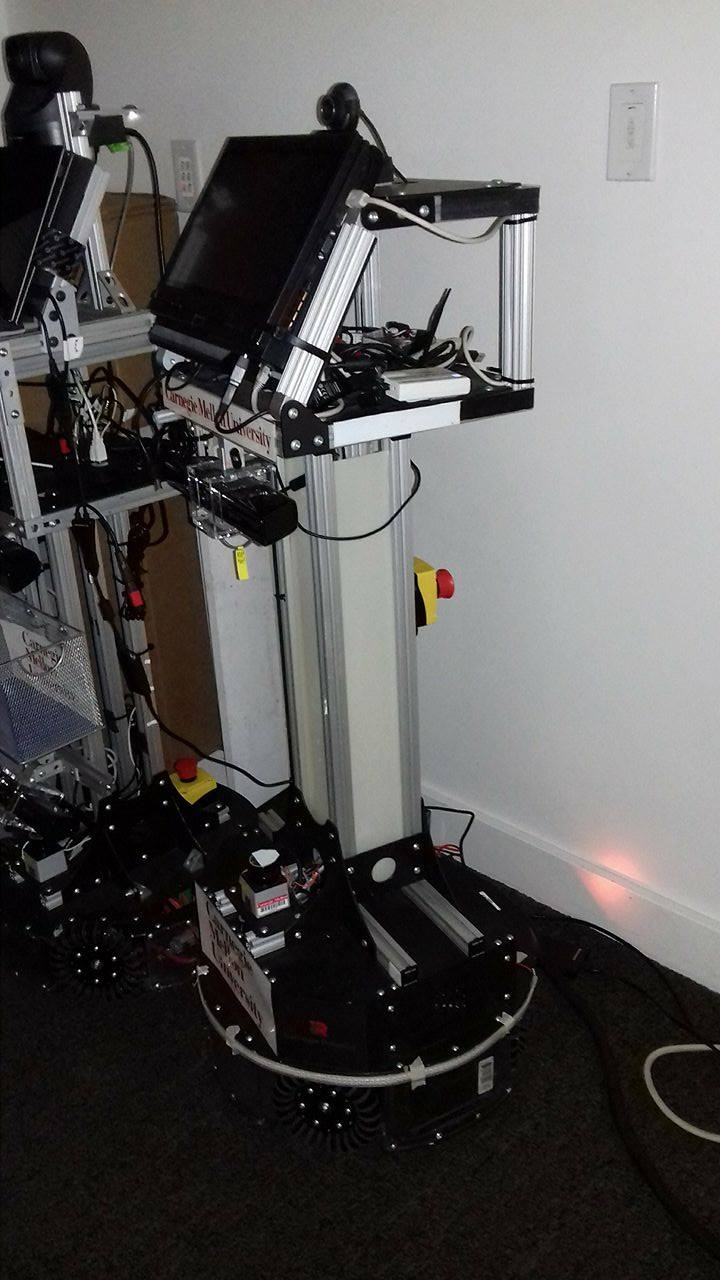
\includegraphics[width=4cm]{images/cobot}
        \caption{Cobot robots that roam around \gls{CMU} Gates' computer science
        building.}
        \label{fig:cobot}
\end{figure}

Moreover, similar work was developed in efficient object search \cite{veiga2016efficient},
by \textit{Veiga et al}. They used probabilistic logic (this was accomplished
while using\textit{Problog}) to represent object locations
as beliefs. Additionaly, the object search decision module was modeled after a
\gls{POMDP}, in order to find objects in the minimum time possible.
The information about the environment was stored in a semantic map and was
updated repeatedly whenever it was acquired new data from sensors. That semantic
map included probabilistic rules to update its knowledge about the environment.
Additionaly, they used an offline \gls{POMDP} solver in order to
make decisions on the environment. Finnaly, they implemented their software pipeline into the 
\textit{Mbot} platform.
In contrast, this work focus on fully integrating \glspl{PLPL} into 
the domain description while dealing with fully observable states. The robotic platform for this
task was the same.

\textit{Antunes et al.} proposed a probabilistic planning approach 
in order to decode human verbal instructions to robot actions \cite{antunes2016human}. 
A pipeline was created which has the following important parts: semantic reasoning for human
verbal instructions; goals and formulation; and robotic actuation. The proposed
architecture was implemented and tested on the \textit{Icub} robotic platform.
This scenario includes multiple sources of knowledge: prior information;
semantic knowledge from verbal instructions; and lastly, knowledge from real
world perception. It uses \textit{PRADA} probabilistic planner as a method to
determine the best grounded action in each possible situation the robot encounters.
In contrast, the system developed here integrates \glspl{DDC} into the domain description.

\textit{Bogdan et al.} used probabilistic programming to learn affordance models which can 
express relations between objects \cite{moldovan2017relational}.
The learned model was then incorporated into a planner in order to solve goals expressed 
in verbal language. They focused on \gls{PLPL} in order to represent real world object 
relations in spite of using something like \glspl{BN} which are unable to represent them. 
For that purpose, they took advantage of \glspl{DDC} from \textit{Nitti et al.} 
\cite{nitti2016probabilistic}. Their pipeline consisted on: first, learning an appropriate
affordance model and then, generalizing it to a state transition model; in order to
finally use it on real world benchmarks by means of a planner. This planner was a naive 
sample based planner without policy improvement. Lastly, their software architecture was 
implemented in the \textit{Icub} robotic platform. The work presented on this dissertation 
builds upon the same \gls{PLPL} from \textit{Nitti et al.} and uses the integrated planner \gls{HYPE}
in order to model and plan in the designed world model. Then, the software architecture is 
implemented on top of the \textit{Mbot} robotic platform.

Finally, the concept of \gls{SA} could be introduced on the recent project about
collaborative robots, the \textit{Space CoBot} project \cite{roque2016space}. The project
aims to integrate collaborative robots in microgravity environments such as the
International Space Station. Tasks on these environments require similar motor and sensorial skills 
as those of domestic robots. However, uncertainty about the robot's surroundings and actions still
exist, and other limitations could harm task performance, in general. \glspl{SA} could be used to
increase task success.
